%%%%%%%%%%%%%%%%%%%%%%%%%%%%%%%%%%%%%%%%%%%%%%%%%%%%%%%%%%%%%%%%%%%%%%%%%%%%%%%%
%2345678901234567890123456789012345678901234567890123456789012345678901234567890
%        1         2         3         4         5         6         7         8
% DOCUMENT CLASS
\documentclass[oneside,12pt]{Classes/RoboticsLaTeX}

% USEFUL PACKAGES
% Commonly-used packages are included by default.
% Refer to section "Book - Useful packages" in the class file "Classes/RoboticsLaTeX.cls" for the complete list.
\usepackage{amsmath}
\usepackage{amsfonts}
\usepackage{algorithm}
\usepackage{algorithmic}
\usepackage{multirow}
\usepackage{colortbl}
\usepackage{color}
\usepackage[table]{xcolor}
\usepackage{epigraph}
\usepackage{graphicx}
%\usepackage{subfigure}
\usepackage{caption}
\usepackage{subcaption}
\usepackage{hyperref}
\usepackage{tabularx}
\usepackage{float}
\usepackage{longtable}
\usepackage[pdftex]{graphicx}
\usepackage{pdfpages}
%\usepackage{tabularx}
\usepackage{pdflscape}
\usepackage{setspace}
\usepackage[utf8]{inputenc}
\usepackage[table]{xcolor}
\usepackage{url}
\usepackage{float}
\usepackage{titlesec}
\usepackage{hyperref}
\setstretch{1.5}
\usepackage{enumitem}
\usepackage{nomencl}
\graphicspath{{C:/Users/CS-Guest-2/Desktop/Nuig/MSc_AI/MSc-AI-SEM2/Final Project/images/}}
%\onehalfspacing
% SPECIAL COMMANDS
% correct bad hyphenation
\hyphenation{op-tical net-works semi-conduc-tor}
\hyphenation{par-ti-cu-lar mo-du-le ge-stu-re}
% INTERLINEA 1.5
%\renewcommand{\baselinestretch}{1.5}

%% ignore slightly overfull and underfull boxes
%\hbadness=10000'
%\hfuzz=50pt
% declare commonly used operators
%\DeclareMathOperator*{\argmax}{argmax}

% HEADER
\title{\Large{Generative Adversarial Network (GAN) for Irish Traditional Music Generation}}

  \author{Tapan Vivek Auti (20231499)}
  \collegeordept{School of Computer Science}
  \university{National University of Ireland, Galway}
  \crest{
\includegraphics[width=75mm]{Figures/logo_NUI.png}}


\supervisor{Prof. Mathieu d'Aquin }
%\supervisor{Name of the Supervisor}
%\supervisor{Name of the Co-Supervisor}	
% \supervisor{Dr. Jane Smith}
% \supervisorSecond{Dr. Mihael Arcan}

% text before "In partial fulfillment of the requirements for the degree of" in .cls file/line 153\
% replace PROGRAMME with Data Analytics, Artificial Intelligence, or Artificial Intelligence - Online
\degree{MSc in Computer Science (Artificial Intelligence)}
\degreedate{August 31, 2021}

%%%%%%%%%%%%%%%%%%%%%%%%%%%%%%%%%%%%%%%%%%%%%%%%%%%%%%%%%%%%%%%%%%%%%%%%%%%%%%%%
%%% uncomment if glossary needed, see examples in file
%\makeglossaries
%\loadglsentries{glossary}
\begin{document}
\begin{spacing}{1}
\maketitle
\end{spacing}
\titleformat{\chapter}[display]
  {\normalfont\huge\bfseries}{\vskip-2.5em\chaptertitlename\ \thechapter}{20pt}{\Large}
\titlespacing*{\chapter}{0pt}{*-2}{*1}



% add an empty page after title page
\newpage\null\thispagestyle{empty}\newpage

% set the number of sectioning levels that get number and appear in the contents
\setcounter{secnumdepth}{3}
\setcounter{tocdepth}{3}

\frontmatter
% replace PROGRAMME with Data Analytics, Artificial Intelligence, or Artificial Intelligence - Online
\textbf{DECLARATION} 
I, TAPAN VIVEK AUTI, do hereby declare that this thesis entitled Generative Adversarial Network (GAN) for Irish Traditional Music Generation is a bonafide record of research work done by me for the award of MSc in Computer Science (Artificial Intelligence) from National University of Ireland, Galway. It has not been previously submitted, in part or whole, to any university or institution for any degree, diploma, or other qualification. 
\newline

\begin{tabular}{@{}p{.5in}p{4in}@{}}
Signature:
\includegraphics[scale = 0.5]{Sign.png} 
\end{tabular}
\newpage


%%%% uncomment if acknowledgements needed
%\textbf{Acknowledgement}
%
%
%\newpage\textbf{}


% THESIS ABSTRACT

\begin{abstracts}

The earliest research can be found around the 1940s and the majority of the Research that emerged over Neural Network and its application can be found after the 1980s. From then to the present, there have been significant changes in the applications and use of Neural Network and the concepts of Deep Learning. Many kinds of research emerged in all the fields about machines showing cognitive abilities, which is not new. The capabilities of performing human tasks and cognitive thinking shown by machines is what debatably AI can achieve and researches in. Over the years the research gave rise to new concepts of reproducing various activities performed by humans, one such being Music.

The concept of music reproduction with the help of deep learning is as well not new, but what is new is the quality of regeneration, its similarities to original work, and also the uniqueness of melodies generated. We can say the machine truly learned and performed, along with all these things one crucial thing that is also new in today's research is the availability of resources. This thesis has tried to achieve one similar thing where I have tried to reproduce Irish traditional folk music.

Generative Adversarial Network model has been proposed for the generation where Long Short-Term Memory (LSTM) will be used as the generator and as the discriminator. ABC files have been used to train the model for music generation. This thesis aims to generate tunes that will be similar to Irish Folk Music with a model that is not specifically tuned for Irish Folk but can later be used on any type of music and generate similar tunes.

\end{abstracts}


\tableofcontents
\listoffigures
%\listoftables

\mainmatter

\chapter{Introduction}
\label{chap:introduction}
\section{Motivation}

The vast applications of Deep Learning in fields of computer vision, analysis, prediction, etc. are no doubt noteworthy but, the implementations and modeling used for the generation as the ones in the WOMBO app for music lip-syncing or Instagram filters have always intrigued me. The power of AI to be used to learn and reproduce something unique yet similar is one of the greatest research goals that we have achieved over the years.

Previously, having seen many applications of Deep Learning used to reproduce melodies of various individual instruments or random noise in form of music made me realize that the scope for this and other variants are unprecedented. Also having a bit of predefined interest for Folk Music I decided to use Traditional Irish Music for my thesis and to reproduce melodies that showed resemblance to the same.

The outcome I wish to achieve, are melodies generated that are not exactly sounding like one of our input songs used or like one copied from the composer directly with some minor changes, but more or less matching the same genre or theme, with the tunes being pleasant to hear and sounding like Irish Traditional Music to people hearing it for the first time. The data and model to be built on should be something that was not exactly done before with the properties of Robustness, Flexibility, and Polymorphic in nature.

\section{Data Used}
For this thesis, I researched various repositories freely available on the internet that had a clear focus on Irish Traditional Music. After thorough research, we decided to go with the repository made freely available by \cite{session}.

The music files available on this site are in ABC format. Normally ABC format is converted into the midi format that is then converted into .wav which we can hear as normal music. A basic ABC file looks like the following.
\begin{verbatim}
X:1
T:Paddy O'Rafferty  
C:Trad.  
M:6/8  
K:D  
dff cee|def gfe|dff cee|dfe dBA|dff cee|def gfe|faf gfe|1 dfe dB
A:|2 dfe dcB|]  
~A3 B3|gfe fdB|AFA B2c|dfe dcB|~A3 ~B3|efe efg|faf gfe|1 dfe dcB:
2 dfe dBA|]  
fAA eAA|def gfe|fAA eAA|dfe dBA|fAA eAA|def gfe|faf gfe|dfe dBA:|
\end{verbatim}
-\cite{abcnotation}

The ABC file has two parts, the header that has all the basic information including various other parameters depending on the type of file and the second part are the notes, In the example above the first five lines are the header and the last 3 lines are the notes.
\begin{verbatim}
X:1 is the reference number,
T: Paddy O'Rafferty, is the Title, 
C: Trad, defines the composer,
\end{verbatim}here it means traditional as the original composer name is lost due to the tune being vintage so it's better to mark this as traditional. This varies according to the creator of the file.
A lot of other features are present but the ones that concern us are only X, M, K, and L where M and K are the meter and key of tune, X contains the reference number that is not that important and L is note length, L being the most important as this will help us split the tune into parts if we want in preprocessing of the data.
More detailed information related to these notations and the type of file is given in Chapter 2 - Background.

In this thesis, we look at producing a GAN model trained on the above dataset to produce strings in ABC notation that can not only be parsed and interpreted as valid music, but also correspond to melodies in the general style of Irish folk music. The Gan model we look to produce will not be limited to this dataset, but can later be used on any type of music and notes with dataset in ABC format.

\section{Flow of Thesis}
\textbf{Chapter 1} - Introduction, gives a brief introduction to the thesis, a generic idea of the data being used, the motivation for the thesis, and the flow of the thesis.

\noindent
\textbf{Chapter 2} - Background, gives thorough information about all the technologies that are being used in this thesis and tries to explain every concept used in brief, along with a detailed explanation of the data being used and any other relevant information related to the dataset.

\noindent
\textbf{Chapter 3} - Related Work, In this chapter I have tried to cover all the prominent researchers from the past that match my work and tried to explain briefly how the advancements were made over the years till now and what their approaches were.

\noindent
\textbf{Chapter 4} - Methodology, In this chapter I have tried to give step by step and detailed information about all the steps conducted to complete the modeling of the thesis and its implementation, right from the data preprocessing to the models used and the training done to achieve results.

\noindent
\textbf{Chapter 5} - Evaluation, In this chapter I have put forward all the technical challenges that I faced while doing the thesis along with its results.

\noindent
\textbf{Chapter 6} - Conclusion and Scope, In this chapter the future scope for improvement and conclusion of the thesis are mentioned in understandable terms.

\chapter{Background}
\label{chap:backg}

\section{Deep Learning}
\cite{ibm} defines deep learning as "Deep learning attempts to mimic the human brain—albeit far from matching its ability—enabling systems to cluster data and make predictions with incredible accuracy."

Deep Learning is a subfield of machine learning that deals with models or algorithms that are such constructed that they mimic the structure of our brain, basically a type of Neural Network with a lot of layers of hierarchy but always not necessarily many, with each level having some sense of abstraction that deals with the huge amount of data and processes it. There are Neural Networks with just one layer too but the addition of layers helps deal with the complexity and to get better results.

The applications of Deep Learning are way beyond imagination and the future scope where we can implement it is without question substantial.

The following is the most basic and simple representation of a Neural Network.

\begin{figure}[H]
  \centering
  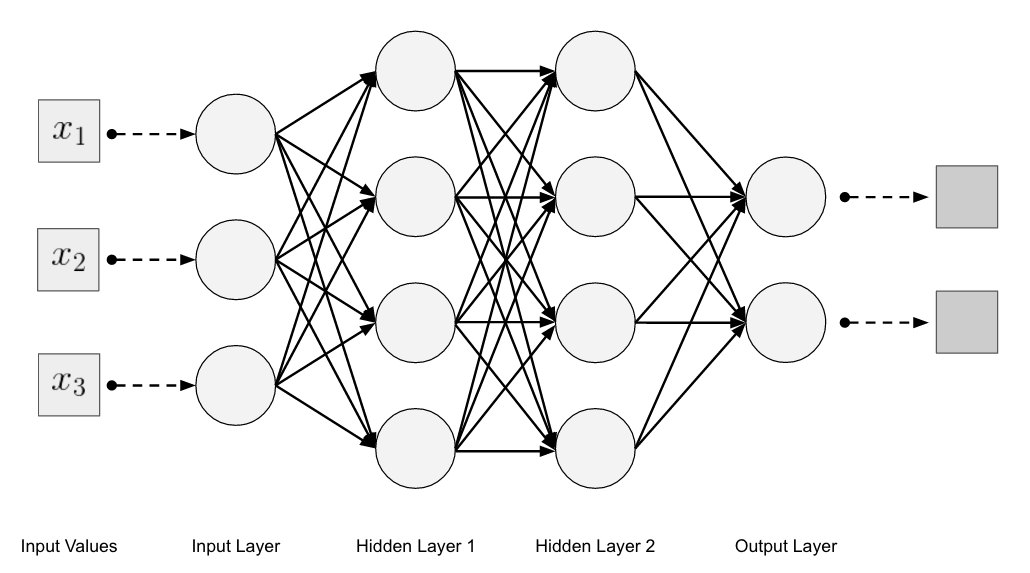
\includegraphics[width=0.80\linewidth]{Figures/dnn.png}
  \caption{Deep Neural Network}
  \label{fig:dnn}
\end{figure}

Deep Learning uses various factors such as inputs, weights, and biases that are processed to get accurate predictions and classifications, etc. The Deep Neural Network has multiple layers and each layer has multiple nodes, these layers are built upon each other to get the most optimized solution.

\section{Recurrent Neural Network}

\cite{ibm}, "A recurrent neural network (RNN) is a type of artificial neural network which uses sequential data or time-series data." Unlike Feedforward Neural Network, RNN has its internal memory, it uses the same function for each input and the output depends on the previous operations, the output produced is then sent back to RNN. It learns from its previous inputs and makes predictions upon them.
\begin{figure}[H]
  \centering
  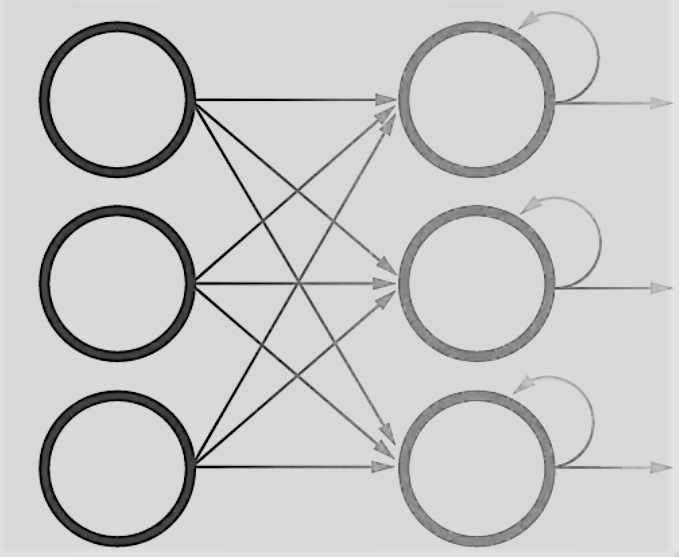
\includegraphics[width=0.5\linewidth]{Figures/rnn.png}
  \caption{Recurrent Neural Network}
  \label{fig:rnn}
\end{figure}
So basically the next step has two inputs, the output of the current state as well as the input of the state and so on. An activation function determines whether the neuron should be activated and it brings the activations to a range depending upon the functions used. The most common functions are-
\begin{itemize}
  \item Sigmoid Function:
  \begin{figure}[H]
    \centering
    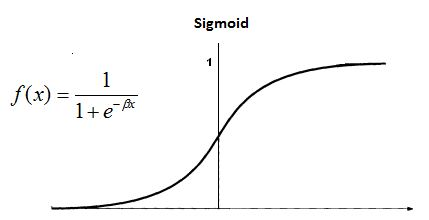
\includegraphics[width=0.5\linewidth]{Figures/sigmoid.png}
    \caption{Sigmoid Function}
    \label{fig:sigmoid}
  \end{figure}

  \item Relu Function:
  \begin{figure}[H]
    \centering
    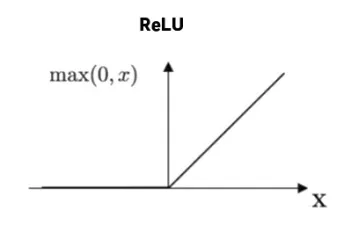
\includegraphics[width=0.5\linewidth]{Figures/relu.png}
    \caption{Relu Function}
    \label{fig:relu}
  \end{figure}

  \item Tanh Function:
  \begin{figure}[H]
    \centering
    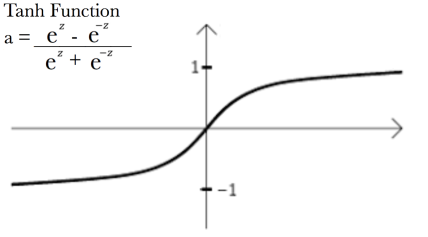
\includegraphics[width=0.5\linewidth]{Figures/tanh.png}
    \caption{Tanh Function}
    \label{fig:tanh}
  \end{figure}
\end{itemize}

\section{LSTM (Long-Term Short Memory)}
LSTM is a popular Recurrent Neural Network(RNN) Architecture, it solves the problem of long-term dependencies of RNN. In cases where the current state's output is being affected by the input of states occurring much earlier in the flow, then in such case, it becomes very hard for the RNN to correctly predict the output and RNN fails. To overcome this LSTM was introduced, it was first used to solve vanishing gradients problems and unlike RNN it has three states, input, output and a forget gate which controls the flow and gives predictions.

\begin{figure}[H]
  \centering
  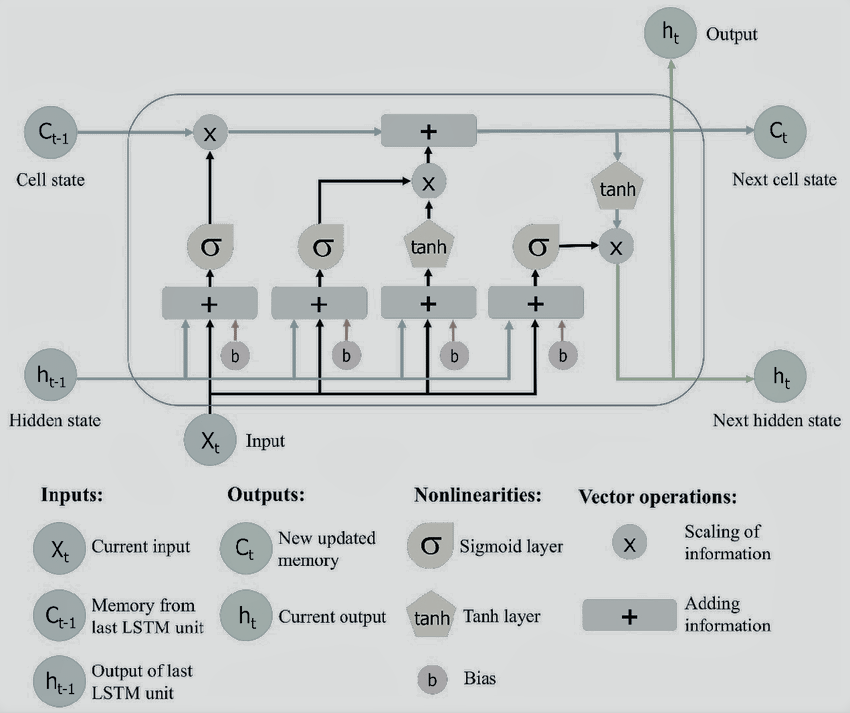
\includegraphics[width=0.90\linewidth]{Figures/lstm.png}
  \caption{LSTM Structure by \cite{yan}}
  \label{fig:lstm}
\end{figure}

\section{CNN (Convolutional Neural Network)}

Three main reasons that make CNN better than any other Neural Network are the convolutional layer, the pooling layer, and the fully connected layer. With each layer the CNN's complexity is increased, the first few layers focus on simple features and the latter on more complex identification, etc. CNN has much greater performance than others concerning image, text, and audio files. The main building block of ConvNets is the convolutional layer, all the main computations occur here. It has 3 main parts i.e. filter, feature map, and the input data. \cite{ibm}

Pooling is downsampling the input and deals with the dimensionality reduction of the parameters from the input. \cite{ibm} There are two main types of pooling, max pooling, and average pooling.

The last Layer is fully connected, this layer all the nodes in the output layer are connected to the previous layer, this is normally the last layer of the model.
\begin{figure}[H]
  \centering
  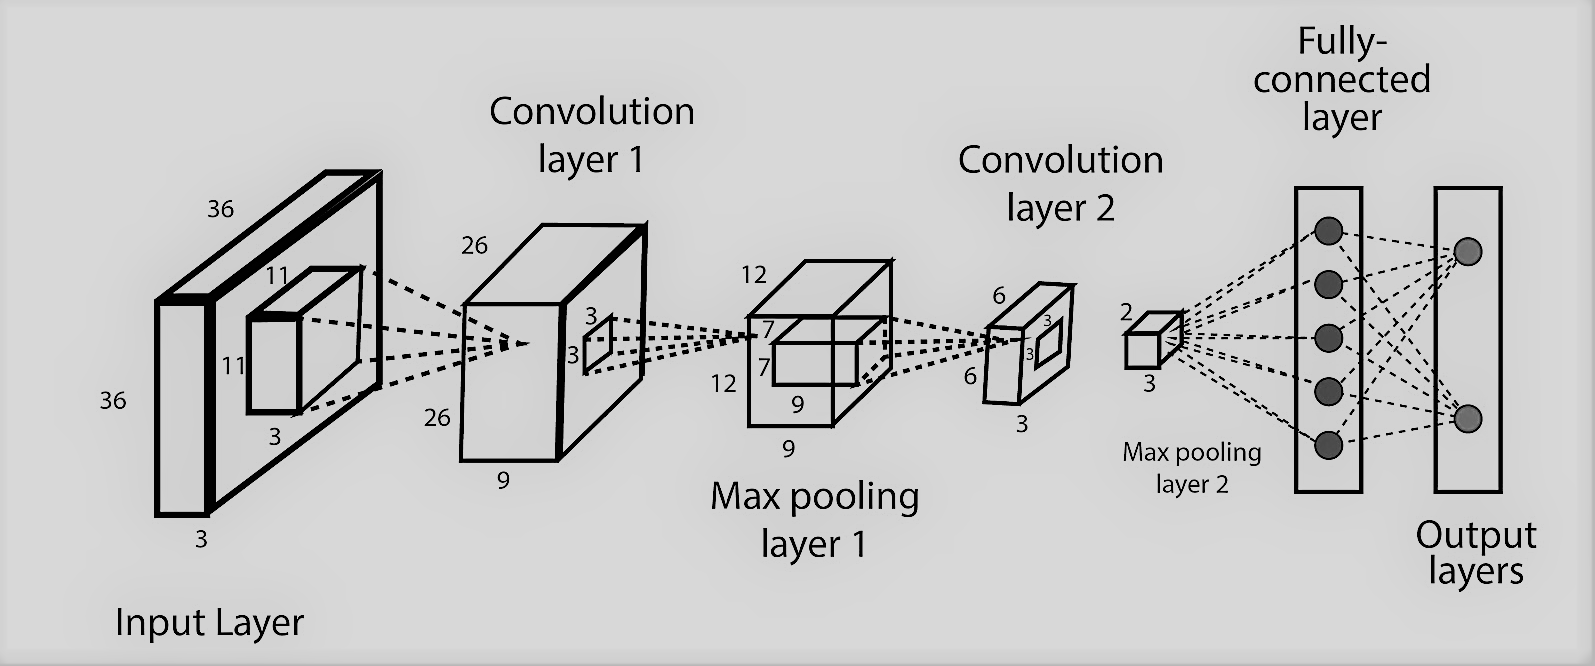
\includegraphics[width=0.90\linewidth]{Figures/cnn.png}
  \caption{ConvNets Architecture by \cite{cnnfig}}
  \label{fig:cnn}
\end{figure}

\section{GAN (Generative Adversarial Netwrok)}


This is a similar concept to that of Convolutional Neural Network, it is a type of generative modeling. Generative modeling is a subfield of machine learning where the features are found and learned automatically from the input data in a way that new output can be generated from the model.

There are two parts of GAN, one being the generator that creates new examples from the data and the discriminator that classifies the data, the job of the generator is to create such examples that the discriminator is not able to identify correctly and discriminator tries to find the real ones and the fake ones. The two models are run simultaneously.

\begin{figure}[H]
  \centering
  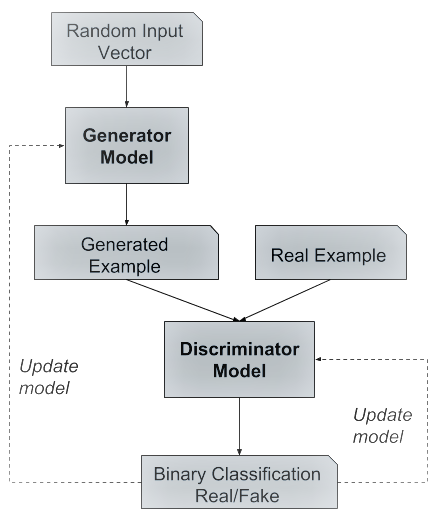
\includegraphics[width=0.5\linewidth]{Figures/gan.png}
  \caption{Architecture of GAN as defined by \cite{brownlee_2019}}
  \label{fig:gan}
\end{figure}

\section{Keras}

\cite{keras} defined "Keras is an API designed for human beings, not machines. Keras follows best practices for reducing cognitive load: it offers consistent and simple APIs, it minimizes the number of user actions required for common use cases, and it provides clear and actionable error messages. It also has extensive documentation and developer guides."

Keras is a deep learning framework focusing on Neural Networks, it uses a python interface for the same. It is mostly used to deal with the various aspects of building models of Neural Network like the layers and functions, it has support to Convolutional and Recurrent Neural Network as well.

\section{Tensorflow}

Tensorflow is more of an open-source library with which we can perform various Machine Learning tasks.

\cite{tensorflow} defined it as "TensorFlow is an end-to-end open-source platform for machine learning. It has a comprehensive, flexible ecosystem of tools, libraries, and community resources that lets researchers push the state-of-the-art in Machine Learning and developers easily build and deploy Machine Learning powered applications."

It gives us the ability to build and train Machine Learning models easily, and also deploy them on the cloud. It was developed by the Google Brain team for internal use and used for research purposes in Google. We can debug and train Keras and TensorFlow code using TensorFlow, it is mostly used for numerical computations using graphs.

\section{Data Representation}

The ABC notations use a-g and A-G, Z for representation of notes and rest, other elements denote the type of notes i.e. sharp, flat, raised, or lower octave, length, and ornamentation.

High notes are depicted with " ' ", and low notes are depicted with ", ". The long notes are shown with dash or hyphen " - ". The bar line \verb+"|"+ is used to separate the bars i.e. the beat of the music.



\chapter{Related Work}
\label{chap:rel_work}

The earliest work which used Neural Network for music composition, analysis, and generation can be found around the late 1980s, \cite{mdolson}. This paper dealt with the traditional ways that were used for music generation, and how Neural Network can be used to help achieve greater results. Here the author used a simple implementation for music generation which used a real-time recurrent learning algorithm to generate four simple rhythms and also explained in-depth about back-propagation and generalization in terms of music generation. 

What has changed from then to today, is the availability of more discrete resources for data gathering and the variations that can be found in the availability and type of data. Before, Musical data was available in nonsymbolic forms i.e. musical notes (polyphonic music), etc. It was very hard to train and was complex in training aspects due to the scarce availability of data. "The availability of resources has paved a new pathway for more advancements in deep learning", \cite{deeplearning}, and hence a lot of research has been conducted since then regarding music generation with Neural Network.

\cite{jpon} suggests that all earlier work was done using a single melody, which means only a single instrument was used or only one note was used to generate music. Piano rolls were amongst the most common ones used. The majority  of the research being conducted for music generation was done using RNN and LSTM,  \cite{lstmtemporal}, \cite{rnnmelodies}, \cite{eck}. \cite{rnnmelodies} did evaluation based on the constraints of the output melodies. They combined different aspects such as pitch, notes and based upon their respective weight defined whether the structure of the melody matched the genre of the song.

The very first one to use RNN was \cite{mozer}. He provided motivation for Eck and Schmidhuber, who later were the first ones to apply LSTM for music generation, \cite{eckschmid}. They thought that the music generated from RNN lacked a definite global structure and that it could not learn an entire musical form, the reason behind that being, the temporary events were not handled well by RNN and hence they thought, to deal with these issues there should be something more discrete, so they used LSTM, as RNN also had other drawbacks like failing at timing, counting and CSL learning which was removed using LSTM. \cite{eck} did the evaluation of the model and generated music by plotting the probability of selection between chords and notes. According to him if the plot shows fixed-length repeated loops then it is aimless music and the one which incorporates several structures is good music.

\cite{abcmusic} did the most significant use of sequential ABC files for music generation using LSTM, they in the paper suggest two models for it, one is Char RNN which uses a single character vocabulary and the other is Folk RNN which used transcription token for a generation. They were the first ones to successfully use ABC files for music generation. They preprocessed and separated tunes based on single and transcription tokens and then passed them to the beforementioned models to obtain two different results. To date the only type of research done on music regeneration was mostly on piano rolls which uses midi files for regeneration, \cite{midinet}, \cite{musegan}. These piano rolls generally comprise tunes from a single instrument and rarely have tunes from multiple instruments. This made a stagnancy in the type of music generated, as more or less the dataset used as input was similar. The models used differ in all papers which give rise to variations in the music produced but still somehow show a sense of similarity when mapped with the melodies. Very few models and papers were such that used a combination of multiple instruments and completely new models which produced unique and never before heard melodies. \cite{abcmusic} evaluated the music generated by two methods, one by doing a statistical analysis that compared the statistical output of the tunes with their training data. In this, they included the modes, meters, pitch, and token length as parameters. The second way was music analysis in which they uploaded their music online and let people decide how it sounded and whether it matched the Genre of the input data used.

\cite{polygan} and various other models were generally polyphonic music generation models. These generated polyphonic music by taking midi files as input. Till late 2018 \cite{crnngan} was the only model that used GAN for music generation. He used midi files as input but had drawbacks of not being able to generate music using priming melody or chord sequences. These were removed in \cite{midinet}. MIDI NET used CNN as their main base model which gave them better results \cite{midinet}. \cite{midinet} purely used only human resources to analyze the melodies generated. They made people hear the music generated by the model and the original input used and asked people if they could differentiate between the genre of the melodies. All the test subjects used were from a musical background.

After various researches, it was proved that CNN is faster than RNN and also easily parallelizable \cite{pxlcnn} before this maximum models used RNN only. All the years of research have a paved path for various genres of music generations, like \cite{edm} that tried to reproduce rhythm patterns of electronic music using GAN. It takes the midi files of EDM and tried to reproduce this music which sounded like one that is produced on a professional instrument and resembled actual EDM to some extent. \cite{edm} used rhythm similarities to distinguish and evaluate their model. They plotted the matrix produced by comparing the Rhythm Patterns. 

Like symbolic data for generation, various studies were also conducted for music generation through nonsymbolic forms such as raw music files and waveforms. \cite{mp3net} was one such successful model that generated music from raw files. They used low convolutional GAN as their base model and achieved a milestone of having extremely low computational power while generation. \cite{mp3net} used three factors for evaluation, the first one was the audio quality and timbre defined by the tonality of the tune, the second was the musicality, this is the rhythmic structure of the tune and the last one was sample diversity based on the tempo.

All the models that used GAN had one major drawback, that due to no or less temporal feature extraction the generated music didn't always sound natural and was unstable to overcome. \cite{dmbgan} proposed a new model that considered temporal features as well and had a self-attention mechanism to enable GAN and introduced a new method of switchable normalization to stabilize network training giving them very good results and music generated being stable and soothing to the ear.

A lot of research is being made in music generation considering various aspects of music such as music generation based upon the genre or feel of the music, one such proposed model is used in \cite{cvaegan}. Here the authors took a dataset that has emotions tagged along with the song in the input files, so while producing output the model trains on basis of the feel of the music and generates music based on what genre you want like rowdy, romance, quiet, majestic, etc. \cite{cvaegan} also used human subjects for identifying the resemblance between the tune and emotions.

\cite{gansynth} was the most recent work that successfully synthesized audio by using wave files as input and using GAN for processing and generation. They used a specific controlled dataset for music generation and were able to achieve great speed which was claimed to be one thousand times faster generation than that of  \cite{wavenet}.

The latest research going on has been on music generation from lyrics, \cite{lstmgan} used LSTM generator and discriminator for generation, wherein the dataset the lyrics are mapped to melodies, but comparatively such data is still very scarce to find and hence the result of the mapping is not melodies to lyrics, i.e. the generated music and lyrics not always correlate and sound good to hear, its very random and doesn't make any sense and generally sounds like music with a lot of noise in it and irrelevant to lyrics.

\cite{GanReels} was the only successful implementation of GAN for reproducing Irish traditional music. They considered the input data as similar to image data and processed it in that way. They treated the data like any other image and used GAN to get their output. They used basic Neural Network in their GAN approach and as input used ABC files but took only reels as their genre of music for implementation.

\chapter{Methodology}
\label{chap:methodology}

\section{Data Procurement}

Jeremy the keeper of the renowned Irish Music Repository The Session provided me with access to all the dump files from the repository, \cite{session}. This gave access to The Session's music repository which consists of forty thousand songs in ABC format. I had the access to the database and GIT where dumps were present. From \cite{database} I was able to extract the music by giving commands similar to ones for extraction from any SQL database, as the data here is stored in a similar format. The files with the same meter setting that was 4/4 were used. In this way, the bar length of the data was the same for all songs which made it is easier to process it. At a single time, the application only shows a thousand lines so I had to customize the rowid to get every data. The command for extraction looked like - " select abc from tunes where meter == "4/4" and rowid between 0 and 1000 ". Similarly, I customized the command for all forty thousand rowid's. 'abc' is the column that has the ABC data, and tunes is the database name. After applying this command the data can be downloaded in CSV or JSON format. For the processing in python, I downloaded forty different JSON files and extracted data from them for further processing.

\section{Data Preprocessing}

One by one the JSON files were stored in a single array where every song was an element in the array. Considering my setting for the songs the total length of the array came to be around 21 thousand, so the total number of songs that were used as music data came to be around 21 thousand songs. The array was tokenized to a single array, where every element was a single character in the song. To clean the data I created a list of characters that I wanted to consider from my data. For this purpose, I ignored any other characters like bar $|$ or colon $:$, etc. from the data. Only those characters were used which mattered the most when producing music and those whose absence wouldn't make the data lose its musical touch. I also thought about the characters whose presence made the data much more complicated and might cause issues while training the model, any such characters were ignored. The final array looked like the following -'a' ,'b' ,'c' ,'d' ,'e' ,'f' ,'g' ,'z' ,'A', 'B', 'C', 'D', 'E', 'F', 'G', 1, 2, 3, 4, 5, 6, 7," ' " ,\verb| | |, \verb| _ | ,\verb| ^ | , '/' , '='. This array was used to match the characters from the input data and any characters outside this scope were ignored.

After filtering the data, the array was converted into a single string of characters. This string was then passed to a sequence creation function. This function converted the data as input data for the model in the type of sequences with the desired shape as required. For preparing the sequences, the first task was to vectorize the input. Basic vectorizing with dictionary was implemented. The sequences were generated in an iterating format and with a length of  '+1'. That means if my string is 'helloworld', then the sequence generator generates sequences like 'hello','ellow' and 'llowo' etc. After vectorizing and sequencing, the data were normalized between values 0 and 1. For normalizing the data a special operation was used. There were two steps involved, one was normalizing and the other de-normalizing. The normalization was done with the equation \\
-1 + 2 * (input - min)/(max-min), \\
where min was the numpy percentile of 5 for the input and max was the np percentile of 95 for input.
Later for de-normalisation the equation used was \\
0.5 * (max - min)*(predictions + 1) + min\\
where predictions is the array of predicted values generated by the generator.

\section{Experimental Setup}

For the smooth transition between multiple modules like TensorFlow, Keras, python, to avoid discrepancy of versions and for the use of GPU runtime for faster processing, Google colab was used. The only setting made was runtime changed to GPU from CPU. 

The data files are stored in google drive from where they are retrieved by glob one by one.
\section{Implementation}

The implementation has major four parts :

\begin{itemize}
  \item Building the generator
\end{itemize}

\begin{itemize}
  \item Building the discriminator
\end{itemize}

\begin{itemize}
  \item Combining the two models
\end{itemize}

\begin{itemize}
  \item Training both the models
\end{itemize}

\subsection{Building the Generator}

The input to the generator is a tensor of shape (?,1,100), 100 being the size of the latent dimension, the output of the model is of shape (?,28,1) where 28 is the length of the unique characters in the data.

\begin{figure}[H]
  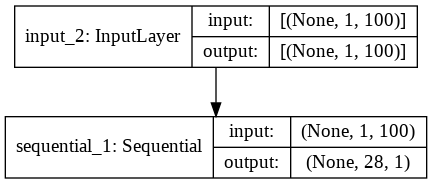
\includegraphics[scale = 0.7]{imagegen}
  \centering
\end{figure}


There are total 7 layers in the discriminator and the model used is LSTM. The structure of the layers is as follows.

\begin{figure}[H]
  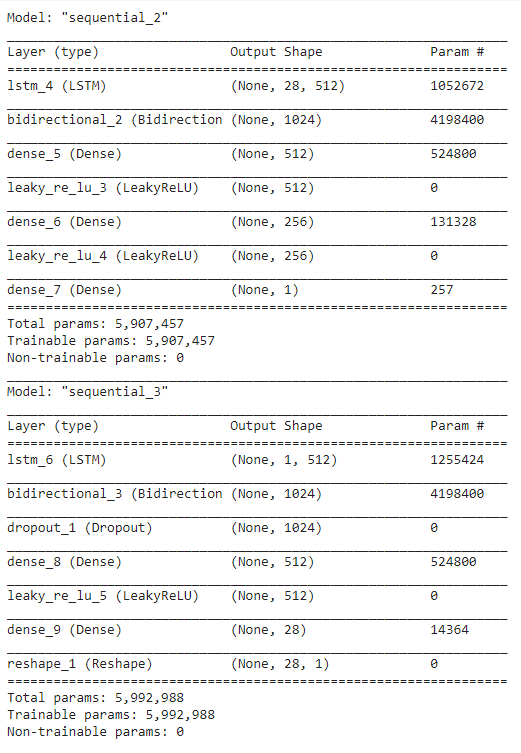
\includegraphics[scale = 1.3]{Capture1}
  \centering
\end{figure}


The first layer of the generator model is a Long Short-Term Memory, this layer has the units set to 512. This means that the dimensionality of the output is set to 512. For this layer, the return sequences are set as True. When the return sequences are set as True that means the hidden state output is returned for each input time step for a single LSTM cell.
For the second layer of the model, I have used a Bidirectional LSTM embedded model. This will generate a copy of each LSTM cell so instead of one LSTM cell there will now be two LSTM blocks beside each other, and one will have the same input while the other will receive input in reverse order.
The next layer is the dropout layer which will set the input to zero randomly which prevents overfitting in the long run.
The next layer is a normal dense layer with 512 units. The dense layers perform the following operation -

$output = activation(dot(input,kernal)+ bias)$

Where kernel is the weight of data and bias is the biased value for optimization.
The next layer is a LeakyRelu activation which is used instead of Relu as Relu is a sparse gradient and LeakyRelu solves the dying Relu problem.
The next layer is again the dense layer with 'tanh' activation and finally ending the model by reshaping it according to the desired input for the discriminator.

After these steps are done, then the model is fully trained and results were generated.

\subsection{Building the Discriminator}

The input to the generator is a tensor of shape (?,28,1), 28 being the size of the unique characters in the data, the output of the model is of shape (?,,1) as the model will predict the output which is a single array.

\begin{figure}[H]
  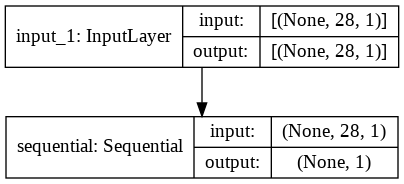
\includegraphics[scale = 0.7]{imagedis}
  \centering
\end{figure}

There are total 7 layers in the discriminator and the model used is LSTM. The structure of the layers is as follows.

\begin{figure}[H]
  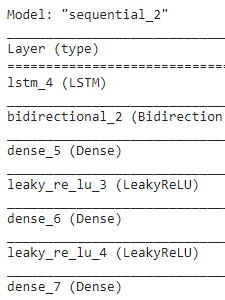
\includegraphics[scale = 1.3]{Capture2}
  \centering
\end{figure}

The first layer of the generator model is a Long Short-Term Memory, this layer has the units set to 512. This means that the dimensionality of the output is set to 512. For this layer, the return sequences are set as True. When the return sequences are set as True that means the hidden state output is returned for each input time step for the single LSTM cell.
For the second layer of the model, I have used a Bidirectional LSTM embedded model. This will generate a copy of each LSTM cell so instead of one LSTM cell there will now be two LSTM blocks beside each other and one will get the same input while the other will receive input in reverse order.
The next layer is a normal dense layer with 512 units. The dense layers perform the following operation 


$output = activation(dot(input,kernal)+ bias)$

Where kernel is the weight of data and bias is the biased value for optimization.
The next layer is a LeakyRelu activation which is used instead of Relu as Relu is a sparse gradient and LeakyRelu solves the dying Relu problem.
The next layer is again the dense layer with 256 units and another LeakyRelu layer.
Finally, the model is ended with the last dense layer which has the activation of 'sigmoid' as this layer will predict whether the data is True or False.

\subsection{Combined Model}

The combined model looks like - 

\begin{figure}[H]
  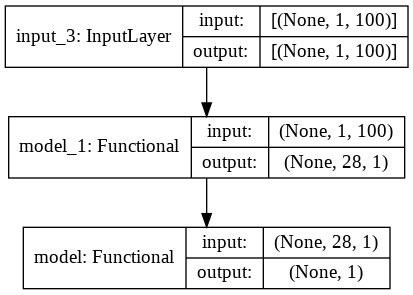
\includegraphics[scale = 0.7]{image}
  \centering
\end{figure}

The generator is given the input of the prepared sequences and the discriminator is given the output of the generator as its input. Later both models are combined by passing the input of generator and output of discriminator to the combined model. The combined model was compiled with 'binary\verb|_|crossentropy' loss and Adam optimizer with a learning rate of 0.0002 and decay rate of 0.5.
The generator and the discriminator are trained separately. Both these models return individual losses. These losses are also used to check the validity of the combined model.

For Discriminator training, first, random noise is generated and this is passed as input to the generator for getting some sequences, these sequences are the generated predictions. Two types of losses are calculated, one is trained on real data that is input data used in the model and the other is trained on the sequences generated by the use of random noise by the generator. The final discriminator loss is the average of these two losses.

For Generator training similar to discriminator first, random noise is generated. This noise is used as input for the combined GAN model on which the training is done and the loss generated is the generator loss. For every epoch, the discriminator and generator loss is calculated and the combined model is improved on every iteration. 

For generating the final output there needs to be some processing involved, for that purpose, after generating random data in the latent dimension and getting the predictions from the generator, the de-normalization step was done and the data was rounded to the nearest even value as the data was in decimals. For that purpose $np.around()$ was used.

The output received is in the format of an array of size 20. That is total of 20 small tunes are generated by the model which can be later converted to ABC format. The array is of integers so the integers are then converted to characters by matching them to dictionary values used before at the time of vectorizing. The array is then converted to a string that looks like -  $FfaddgbcFg^2G2gggeg2f2g2f2gg$

\chapter{Evaluation}
\label{chap:eval}

\section{Challenges}

The most difficult task is data gathering. Even though there are many repositories freely available with a sufficient amount of data present, the songs are not always in good format or standards. Very few repositories have stored the songs in ABC format and not all are open to the public. \cite{session} has all their songs in ABC format. The issue with open repositories is that anyone can freely upload the song there, so it might be the case that many rookies in music are uploading songs that are not always good. The songs are uploaded in .wav format and are later converted to ABC format. While converting it may also happen that the song is not converted properly. While going through a few songs I found that the ABC files have sometimes unwanted characters and other information written in them like the Meter of song or release year. It is not possible to clean forty thousand songs by going through them one by one and checking if ABC is correct and removing unwanted data manually from it. Even writing a script for it is very complex, as ABC format itself is very complex and can have many settings with tons of different characters. The major issue faced here was to do that in a small timeframe. It was not possible to spend so much time on data preprocessing and cleaning, so in this thesis, the data is considered as correct and used as is with whatever cleaning possible.

The database in which the songs are stored gave access to download either JSON file or CSV file. The JSON file took new lines and spaces as well into coding conversions which made the data extraction from JSON files also a difficult task and the CSV file takes weird characters while converting the table into CSV format. The whole data without any removal of characters was having 120 unique tokens and while preparing sequences of that huge amount of data which was nearly 40 thousand songs, the GPU of google colab was crashing as the processing was exceeding the limit of 12 GB RAM. So to fix this, the data was reduced(sorted based on meter type) and instead of passing an array to the sequence generator, the string was passed which reduced the memory size and processing complexity.

The normalization of data was not done before, but that generated vague predictions and the random input which was initially passed didn't match the data. Even after doing normalization converting the data back again into a readable format that is de-vectorizing was extremely difficult as reverse-engineering the vectorizing didn't produce results for de-vectorization. So trial and error took a lot of time and effort to finalize the vectorizing and de-vectorizing of equations.

\section{Results}

After training the model on the data for 4000 epoch the loss and accuracy of the model were as follows :

\begin{figure}[H]
  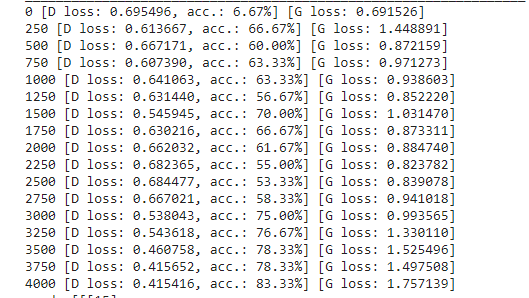
\includegraphics[scale = 1.2]{Capture}
\end{figure}

After viewing the losses and the accuracy we can see 3 traits that make this GAN model a good one.

\begin{itemize}
  \item The first thing is that the discriminator loss has an average loss of around 0.5 which is good as that is calculated based on the real and the fake sequences so the loss coming around half is expected. 
\end{itemize}

\begin{itemize}
  \item The second thing is the accuracy of the discriminator is around 70 -80 percent and is getting stable at that slab after 3000 epoch.
\end{itemize}

\begin{itemize}
  \item The generator loss is calculated with every iteration based on the combined model so for every good generated data the positive loss is added to the model so a loss above 1.5 is a sign of good model and data.
\end{itemize}

\begin{itemize}
  \item After reviewing all the above three mentioned points we can say that the model is not converging as convergence leads to the generator getting trained on bad data which will later make generated sequences similar to noise sequences and the model will not be trained properly.
\end{itemize}

The graph for the same that is losses over 4000 epoch is plotted as follows:

\begin{figure}[H]
  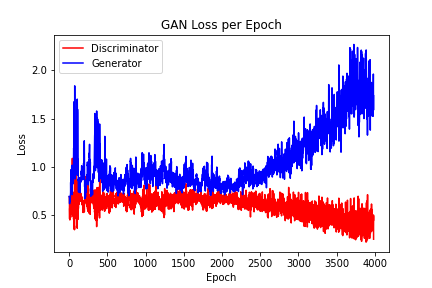
\includegraphics[scale = 1.2]{loss}
\end{figure}

The model successfully generated 20 songs of small length. Out of those twenty songs fourteen such songs were so perfect that they could be easily converted to .wav form without any manual changes. Out of the remaining 6, 2 songs were error-free but they couldn't be converted and 1 song has too many long notes and 2 had an ending not appropriate.

After studying the 3 faulty songs I got to know that this was caused due to discrepancies in the input data as mentioned earlier and breaking of songs into a single string and sequences sometimes disrupted the syntax of ABC files. The model is trained to only predict the ABC file with data and the parameters needed for converting the data are manually added. These include the title that is X and the meter of the songs which is standard that is $M:4/4$. 
The successfully generated ABC files are mentioned below:

\begin{itemize}
  \item \verb|Ef^ggga=A2C=B3d2fff2f3gdg_fg|
\end{itemize}

\begin{itemize}
  \item \verb|fagdf_f2fc_Gc_=cDbDc7gc3aA3d|
\end{itemize}

\begin{itemize}
  \item \verb|ggggggeDa4d2e^f2fffgbebedefd|
\end{itemize}

\begin{itemize}
  \item \verb|FfaddgbcFg^2G2gggeg2f2g2f2gg|
\end{itemize}

\begin{itemize}
  \item \verb|^DEDDCEEE6E_FDGBE7E_FDEDCECC|
\end{itemize}

\begin{itemize}
  \item \verb|=FaabEb2af^eff_gbg^aFgfCcfFC|
\end{itemize}

\begin{itemize}
  \item \verb|gaf6_fae^=EdD=B^DEaAcBd_aAdf|
\end{itemize}

\begin{itemize}
  \item \verb|AB3ggfd3^gf2g=^2ag546fcfbf5a|
\end{itemize}

\begin{itemize}
  \item \verb|fcf__gFfD3Gfa_G^_eebdCbaEcfd|
\end{itemize}

\begin{itemize}
  \item \verb|fb5aFfdbcgc6fdggeEgfDdD2==GC|
\end{itemize}

\begin{itemize}
  \item \verb|e_eec3F2G2aa_Fc2F7cc_fcgGb7e|
\end{itemize}

\begin{itemize}
  \item \verb|=F=DG2CeE_BBEE^DA4D^^a_gcGb4|
\end{itemize}

\begin{itemize}
  \item \verb|FFf6ef_7^ADdFDB3C^5=C^aeEBAD|
\end{itemize}

\begin{itemize}
  \item \verb|ggggfgEea4fgggggggggfgg2g2gg|
\end{itemize}

Randomly selected 5 generated songs along with 5 songs from the input data were played to a group of 20 people. Out of those 20 people, 6 were familiar with Irish traditional music and 4 were from a musical background.

They were told to do the evaluation based on 3 things, the first being, did the songs sound like music to them? Second, which of those sound like ones played by a machine? And third, do all the songs sound similar in category and genre, and if they sound like folk music? Their answers were collected and converted to a percentile based on the information mentioned above. 

For the first question they were made to hear only the generated songs, 85\% of the people thought that the songs sound like music to them and all the 4 people from the musical background were also in this mentioned percentile.

For the second question 60\%, people guessed the songs played by machines incorrectly and were not able to differentiate between human and machine-generated songs.

For the third question 70\%, people thought that all the songs belong to the similar background and can be classified into some sort of Irish Music. Out of the 6 people familiar with Irish music 4 thought that the music generated by the model can be classified as something similar to Irish Folk.

\chapter{Conclusion and Future Scope}
\label{chap:scopeandcon}

\section{Conclusion}

After reviewing the evaluation and results, I can say that the output satisfies my goal of the thesis to the maximum extent. The songs were generated successfully and they sound like parts of Irish Music, along with this the GAN model is also accurate and can later be used without any changes for any other type of musical data.

To conclude I can say that the research of the thesis is successful but, with more time and effort the model and the songs can be made better and the generation length of the songs could be increased to generate full-length songs.
\section{Future Scope}

\begin{itemize}
  \item Foremost the data used should be more accurate and if possible gathered from resources that have music generated by purely professionals so the data is without any discrepancy. More than 70\% problems that were faced in this thesis could be removed with just the data being good enough.
\end{itemize}

\begin{itemize}
  \item LSTM was tried with GAN first time which gave good results so an improvised model could provide more accurate results with very minimal data cleaning.
\end{itemize}

\begin{itemize}
  \item For this purpose only a few characters from the dictionary were considered for the training of the model, with an improvised model and good data all the characters can be used to get the prediction which will make the songs produced exactly similar to those played by professionals.
\end{itemize}

\begin{itemize}
  \item Right now only the ABC data is taken but with a more improved model the whole data that is one along with the Meter, Mode, and all such parameters could be passed to produce songs with all the parameters included so just converting will suffice and no manual addition would be required.
\end{itemize}

\begin{itemize}
  \item Lastly, even though I'm currently using data with all genres of songs, I don't have the feature to give the type of music while generation. If the model had this capability then I can specify which type of music or other parameters I want my music to be generated in.
\end{itemize}
%%%%%%%%%%%%%%%%%%%%%%%%%%%%%%%%%%%%%%%%%%%%%%%%%%%%%%%%%%%%%%%%%%%%%%%%%%%%%%%%
\bibliographystyle{plainnat}                  % to give author-year style
\renewcommand{\bibname}{References}           % change default name Bibliography to References
\bibliography{references}                     % References file, references.bib
\addcontentsline{toc}{chapter}{References}    % add References to TOC


%%% uncomment if Appendix needed
\appendix
\chapter{Code} 

Please find the code for this thesis at the following link - \href{https://github.com/tapanauti/MSC_Thesis/blob/main/Final_thesis.ipynb}{Code}.

\chapter{Generated Music} 

The midi files are stored in the drive, please follow the link to listen to the music generated - \href{https://drive.google.com/drive/folders/14EMRpjFe9Wrr2mMnjLbV1q08sLtNSFwh?usp=sharing}{Songs}.

\end{document}
